\section{Result}
This section covers the results of this project. It will explain, how the final workflow works and what kind of product were produced during the time of this bachelor thesis.

\subsection{Discussion}
\label{sub:Discussion}

\subsection{Workflow}
During the time of this project, we tried out different algorithms and processes (Section~\ref{sub:Discussion}), to create a workflow, which solves the stated task (Section~\ref{sub:ProblemDescription}).

\begin{figure}[H]
	\centering
	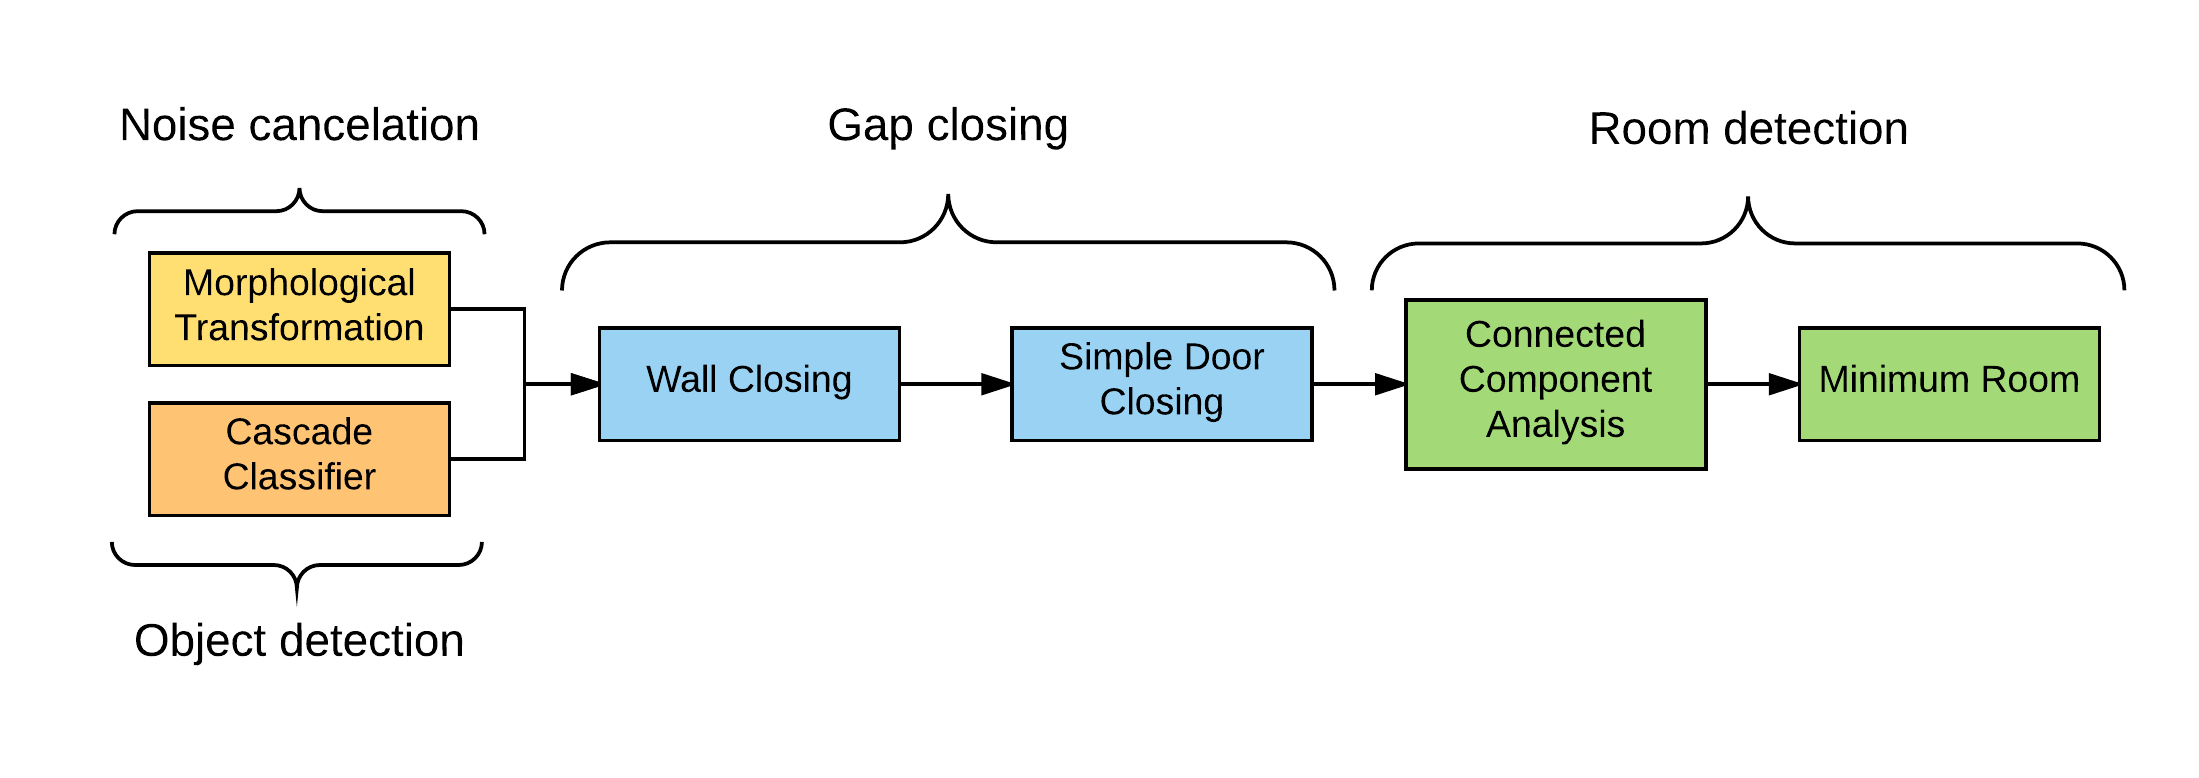
\includegraphics[width=1.0\textwidth]{FinalWorkflow}
	\caption{Final workflow flowchart.}
	\label{fig:FinalWorkflow}
\end{figure}

The workflow is visualised in figure~\ref{fig:FinalWorkflow} and is the same workflow as the workflow three, described in section~\ref{sub:workflow3}. It starts with the object detection (Section~\ref{sub:ObjectDetection}), which detects all doors on a floor plan. This information is saved into the meta image format (Section~\ref{sub:MetaFormat}) for further processing. Then the noise cancelation (Section~\ref{sub:NoiseRemoval}) removes noise like 


\subsection{Prototype}

\subsection{Limitations and restrictions}